\subsection{Chorus and Flanger Effect}

The chorus effect is obtained when a signal is delayed and then mixed with its original version \citep{chorus_gibson} \citep{chorus_apple}. \\
The chorus effect takes a single audio signal as input and applies different delay values to it. Chorus effect can be applied using one delay. Each of the delayed signal are then mixed with the original audio input. \\
A \gls{lfo} can be used to make the delay times vary. Different \gls{lfo}s can be used for each of the delay channels to make a richer sound mix and avoiding repetitive sound but it implies more computations. The same \gls{lfo} can be used for all the delay channels but not at the same cycle for each delay \citep{chorus_testtone}. \\ 

Different parameters on the chorus effect can changed by settings on the hardware. Some of these are:\\
\begin{itemize}
\item \textbf{Delay time}: The time difference between the original sound and the delayed one (The frequency of the signal from the \gls{lfo}).
\item \textbf{Chorus size}: The number of delayed sounds that will be mixed.
\item \textbf{Depth}: The amplitude of the signal from the \gls{lfo}.
\item \textbf{Waveform}: The waveform of the signal from the \gls{lfo} can be changed to triangle, sine, log ect. \citep{hobby_hour_chorus}
\item \textbf{Gain}: The amplification of the delayed signal.
\end{itemize} \citep{chorus_parameters}

The flanger effect is the same as the chorus effect but with shorter delay times and a feedback \citep{chorus_testtone}.

A block diagram for  the chorus effect is shown in \autoref{fig:chorus_diag}.

\begin{figure} [htbp!]
	\centering
\begin{picture}(0,0)%
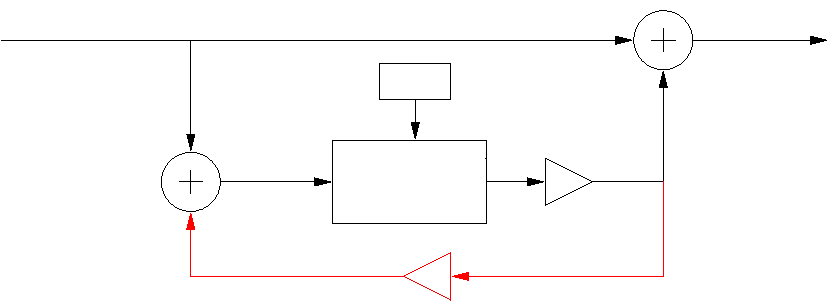
\includegraphics{chorus_diag.pdf}%
\end{picture}%
\setlength{\unitlength}{4144sp}%
%
\begingroup\makeatletter\ifx\SetFigFont\undefined%
\gdef\SetFigFont#1#2#3#4#5{%
	\reset@font\fontsize{#1}{#2pt}%
	\fontfamily{#3}\fontseries{#4}\fontshape{#5}%
	\selectfont}%
\fi\endgroup%
\begin{picture}(6327,3018)(3766,-3493)
\put(6706,-1366){\color[rgb]{0,0,0}LFO}%

\put(8101,-1636){\color[rgb]{0,0,0}Gain}%

\put(3781,-646){\color[rgb]{0,0,0}Input}%

\put(9406,-646){\color[rgb]{0,0,0}Output}%

\put(6571,-1906){\color[rgb]{0,0,0}Delay}%

\put(6616,-3211){\color[rgb]{1,0,0}Delay}%

\put(8101,-2986){\color[rgb]{1,0,0}Gain}%

\put(6706,-2671){\color[rgb]{1,0,0}LFO}%

\end{picture}%



\caption{Block Diagram of the chorus effect.}
\label{fig:chorus_diag}
\end{figure}


As it can be seen on the block diagram in figure \autoref{fig:chorus_diag}, a signal that hasn't been affected by any changes is added to the same signal delayed, controlled by the \gls{lfo}. The addition is done just before the output. This represents the chorus effect \citep{chorus_projectpaper}, and is the black text and drawing. When the red drawing and text is included, it represents the flanger effect. In \autoref{fig:chorus_and_flanger_time} the impulse response of the chorus and the flanger effect. Its is seen that with a pulse as the input, in the chorus effect, the output will be the original pulse, followed by an echo. The period before this echo arrives varies, based on the \gls{lfo}. When using the flanger effect several echoes will arrive, still with varying delay time. 

\begin{figure}[htbp!]
\centering
\def\svgwidth{\columnwidth}
\scalebox{0.8}{\input{figures/analysing/chorus_and_flanger_time_domain.pdf_tex}}
\caption{Impulse response of the chorus effect (black) and the flanger effect (red).}
		\label{fig:chorus_and_flanger_time}
\end{figure}










